% square pyramid P-ABCD, O center, PO height; AC diagonal hidden
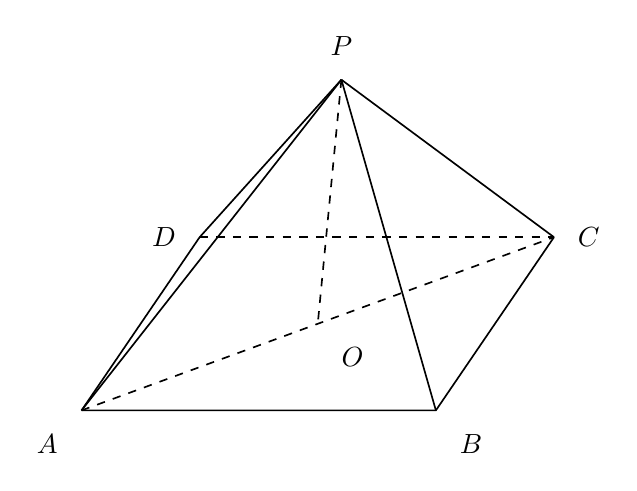
\begin{tikzpicture}[x=1cm,y=1cm,line width=.6pt, font=\normalsize]
  \coordinate (O) at (0,-0.1);
  \coordinate (A) at (-3,-1.2);
  \coordinate (B) at (1.5,-1.2);
  \coordinate (C) at (3,1.0);
  \coordinate (D) at (-1.5,1.0);
  \coordinate (P) at (0.3,3.0);
  % base front/side visible
  \draw (A) -- (B) -- (C);
  \draw (D) -- (A);
  % base back hidden
  \draw[dashed] (D) -- (C);
  % lateral edges
  \draw (P) -- (A);
  \draw (P) -- (B);
  \draw (P) -- (C);
  \draw (P) -- (D);
  % height and diagonal hidden
  \draw[dashed] (P) -- (O);
  \draw[dashed] (A) -- (C);
  \node[above=5pt] at (P) {$P$};
  \node[below left=5pt] at (A) {$A$};
  \node[below right=5pt] at (B) {$B$};
  \node[right=5pt] at (C) {$C$};
  \node[left=5pt] at (D) {$D$};
  \node[below right=5pt] at (O) {$O$};
\end{tikzpicture}
